\part{Foundations}\label{part:foundation}
Zero Knowledge Proof (ZKP) systems are a relatively recent research topic: while the idea in itself,
like many other beautiful ideas, is simple and elegant, its formalization, and even more so its 
realization, is all but trivial.
A first rigorous description of what it means for a proof system to be \emph{Zero Knowledge} was
given by S.\ Goldwasser, S.\ Micali and C.\ Rackoff in 1985~\cite{GoldwasserMR1989} (the work was 
later updated in 1989).

To fully understand the properties of ZKP system, one needs to have an understanding of both 
fundamental and more advanced notions from the fields of group theory, computational theory and 
cryptographical theory. 
This is even more necessary for ZK-SNARK systems and ZK-friendly hash functions.
For this reason, in this first part of the work we will (hopefully) give an exhaustive description
of the tools required to have a better grasp of the results that will be presented in the 
second part.
\chapter{Mathematical Background}\label{chap:math}
In this chapter we will introduce all the mathematical concepts behind ZKP and ZK-friendly 
functions.
While we decided, for completeness, to include even some of the more fundamental notions, we still
expect the reader to have at least a rough idea of these concepts.
\Cref{sec:prime_fields} will introduce prime fields, cyclic groups other related notions.  

\section{Finite algebra}\label{sec:prime_fields}
In algebra, a \emph{tuple} consisting of one or more \emph{sets} together with one or more 
\emph{operations} over the sets is called an \emph{algebraic structure}.
Such structures can be organized according to a quite wide taxonomy, depending on whether 
they satisfy certain properties or not. 
We will denote sets with capital letters (e.g.\  \(S, T, U, \dots \)), a generic operation with a 
circled dot \(\odot \) and algebraic structures with blackboard bold letters 
(e.g.\  \(\mathbb{A}, \mathbb{B}, \mathbb{C}, \dots \)).
We will also denote elements of a set with lowercase letters (e.g.\  \(a, b, c, \dots \)) and 
variables over a set with lowercase letters (e.g.\  \(x, y, z, \dots \)).
Finally, we will often use the term algebra to mean algebraic structure, whenever we belive the 
meaning to be clear from the context.
\begin{remark}
  Some symbols will be reserved to denote some common algebraic structures. 
  In particular, \(\mathbb{B}\) will denote the boolean algebra, while \(\mathbb{N}, \mathbb{Z}, 
  \mathbb{Q}, \mathbb{R}\) and \(\mathbb{C}\) will denote, respectively, the 
  natural, integer, rational, real and complex numbers.
\end{remark}

We will denote the \emph{cardinality} of set \(S\) with \(\abs{S}\), and use the same notation for the \emph{order} of an algebraic structure and for the \emph{arity} of an operation: for example, if \(\odot \) is a binary operation, like integer 
addition\footnote{if considered as a relation, addition would be ternary.}, then 
\(\abs{\odot} = 2\).
When an algebraic structure \(\mathbb{A}\) has exactly one \emph{underlying set} \(A\), we will identify the two, e.g.\ by writing \(x \in \mathbb{A}\) to mean \(x \in A\).

\begin{definition}[Finite algebra]
  A finite algebra is an algebraic structure \(\mathbb{A}\) such that \(\abs{\mathbb{A}} \in \mathbb{N}\).
\end{definition}
\begin{definition}[Subalgebra]
  An algebraic structure \(\mathbb{A} = \Tuple{A, \odot_1, \dots, \odot_n}\) is a subalgebra of an algebraic structure \(\mathbb{A}' = \Tuple{A', \odot'_1, \dots, \odot'_m}\), for some \(n \le m\), if \(A \subseteq A'\) and \(\forall i \le n\colon \odot_i \subseteq \odot'_i\).
\end{definition}

Elements of differents algebraic structures can be associated through \emph{morphisms}.
\begin{definition}[Homomorphism]
  Given two algebras \(\mathbb{A} = \Tuple{A, \odot_{1}, \dots, \odot_{n}}\), 
  \(\mathbb{A}' = \Tuple{A', \odot'_{1}, \dots, \odot'_{n}}\) such that 
  \(\forall i \le n\colon \abs{\odot_i} = \abs{\odot'_i} = a_i\), an homomorphism is a map 
  \(h\colon A \to A'\) such that:
  \begin{align*}
    & \forall i \le n, \forall x_1,\dots, x_{a_{i}} \in A\colon 
    h(\odot_{i}(x_{1}, \dots, x_{a_{i}})) = \odot'_{i}(h(x_{1}), \dots, h(x_{a_{i}})) && 
    \textnormal{(linearity)}
  \end{align*}
  We say that \(\mathbb{A}\) is homomorphic to \(\mathbb{A}'\) through \(h\).
\end{definition}

\begin{definition}[Isomorphism]
  An isomorphism is a bijective homomorphism.
\end{definition}

Given two algebras \(\mathbb{A}\) and \(\mathbb{A}'\), if they are isomorphic through some map
\(h\), we write \(\mathbb{A} \cong_h \mathbb{A}'\), or more succintly \(\mathbb{A} \cong \mathbb{A}'\).

\begin{definition}[Endomorphism, Automorphism]
  An endomorphism is a homomorphism from an algebraic structure \(\mathbb{A}\) to itself.
  An automorphism is an endomorphism which is also an isomorphism.
\end{definition}

\subsection{Groups}
We will now introduce some important classes of algebraic structures equipped with one fundamental 
operation. 
\begin{definition}[Monoid]
  A monoid is a pair \(\mathbb{M} = \Tuple{M, \odot} \), where \(M\) is the 
  underlying set and \(\odot\colon M \times M \to M\) is the \emph{composition} 
  operation, such that the following properties are satisfied: 
  \begin{align*}
    & \forall x,y \in M\colon x \odot \Parens*{y \odot z} = \Parens*{x \odot y} \odot z
      && \textnormal{(\emph{associativity})} \\
    & \exists \algid \in M\colon \forall x \in M\colon x \odot \algid = x
      && \textnormal{(\emph{identity element})}
  \end{align*}
  \(\mathbb{M}\) is a \emph{commutative (or abelian) monoid}, if it also holds that:
  \begin{align*}
    & \forall x,y \in M\colon x \odot y = y \odot x && (\emph{commutativity})
  \end{align*}
  Finally:
  \begin{equation}\label{eq:exponentiation}    
    \forall x \in \mathbb{M}, \forall k \in \mathbb{N}\colon x^{k} = 
    \begin{cases}
      \algid & k = 0 \\
      x^{k-1} \odot x & k > 0
    \end{cases}
  \end{equation}
\end{definition}

\begin{definition}[Cyclic Monoid]
  A cyclic monoid is a monoid \(\mathbb{M} = \Tuple{M, \odot}\) which has a 
  \emph{generator element} \(g\) such that:
  \[\mathbb{M} = \gengroup{g} = \Tuple{\Set{g^k \mid k \in \mathbb{N}}, \odot} \]
\end{definition}

\begin{definition}[Group]
  A group is a monoid \(\mathbb{G} = \Tuple{G, \odot} \), such that: 
  \begin{align*}    
    & \forall x \in G\colon \exists x^{-1} \in G\colon x \odot x^{-1} = \algid
    && \textnormal{(\emph{inverse element})}
  \end{align*}
  With the notion of inverse element, we can rewrite and extend \Cref{eq:exponentiation} 
  for groups as follows:
  \[
    \forall x \in \mathbb{G},\forall k \in \mathbb{Z}\colon x^k =
    \begin{cases}
      x^{k-1} \odot x & k \ge 0 \\
      x^{k+1} \odot x^{-1} & k < 0
    \end{cases}
  \]
  If \(\mathbb{G}\) is also a commutative (resp.\ cyclic) monoid, then it is a 
  commutative (resp.\ cyclic) group.
\end{definition}

The identity element \(\algid \) of a monoid is typically denoted with \(1\) in 
numeric algebras, when the composition operation resembles standard multiplication, or by \(0\) 
when the composition operation resembles standard addition. 
We use the notation \(\algid_{\mathbb{A}}\) (or \(1_{\mathbb{A}}\), 
\(0_{\mathbb{A}}\)) to specify the algebra over which we intend to pick the identity element, 
dropping the subscript when \(\mathbb{A}\) is clear from the context.

It is important to stress that one should be careful not to confuse the symbol and the name of an 
operation or of a special element with its semantics: the syntax to denote the inverse element 
\(x^{-1}\) of a group is reminiscent of standard multiplication inversion, but this is not the 
case in general.
In fact, when the composition operation resembles standard addition, the inverse is more likely 
denoted with \(-x\).
With this clear in mind, to slim the notation we will often be using the same symbols to denote 
even quite different operations (`overloading'), whose semantics should be clear from the 
associated operands. 
\begin{example}
  The algebra \(\mathbb{A} = \mathbb{Z} \setminus \Set{\times}\) (i.e.\ integer numbers 
  without multiplication) is an abelian group: 
  addition is associative and commutative, the identity element is 
  \(\algid_{\mathbb{A}} = 0\), and every number \(x\) has an inverse \(x^{-1} = -x\) 
  (e.g.\  \({42}^{-1} = -42\)). 
\end{example}

\begin{example}\label{ex:endo_group}
  Given a commutative group \(\mathbb{G} = \Tuple{G, \odot}\), consider the algebra 
  \(\Endset{\mathbb{G}}_{+} = \Tuple{H, +}\), where \(H\) is the set of endomorphisms over 
  \(\mathbb{G}\) and \(+\colon H \times H \to H\) is such that 
  \(\forall h_1, h_2 \in H, \forall x \in G\colon \call{\Parens*{h_1 + h_2}}{x} = 
  \call{h_1}{x} + \call{h_2}{x}\).

  \(\Endset{\mathbb{G}}_{+}\) is a commutative group: \(+\) is both associative and 
  commutative, the identity element is \(\algid_{\Endset{\mathbb{G}}_{+}} = z\), where
  \(z\) is the zero endomorphism (i.e.\  \(\forall x \in G\colon \call{z}{x} = 
  \algid_{\mathbb{G}}\)); finally, every homomorphism \(h \in H\) has an inverse 
  \(h^{-1} = -h\) such that \(\forall x \in G\colon \call{\Parens*{-h}}{x} = 
  \call{h}{x}^{-1}\) (in this example, using the \(h^{-1}\) notation causes confusion with 
  the inverse function!).
\end{example}

\begin{example}\label{ex:endo_monoid}
  Consider now the algebra \(\Endset{\mathbb{G}}_{\circ} = \Tuple{H, \circ}\) 
  where \(\mathbb{G}\) and \(H\) are defined as in \Cref{ex:endo_group}, and 
  \(\circ\colon H \times H \to H\) is defined as function composition: 
  \(\call{\Parens*{h_1 \circ h_2}}{x} = \call{h_1}{\call{h_2}{x}}\).
  
  \(\Endset{\mathbb{G}}_{\circ}\) is a monoid: function composition is associative, and the 
  identity element is \(\algid_{\Endset{\mathbb{G}}_{\circ}} = \fooid \), where \(\fooid \) is the
  identity endomorphism (i.e.\  \(\forall x \in G\colon \call{\fooid}{x} = x\)). 
\end{example}

\subsection{Fields}
Many algebraic structures rely on two fundamental operations, called \emph{addition} and 
\emph{multiplication}: two important types of such structures are \emph{rings} and \emph{fields}.
\begin{definition}[Ring]
  A ring is a triple \(\mathbb{O} = \Tuple{O, \oplus, \otimes}\) where \(O\) is the 
  underlying set, \(\oplus\colon O \times O \to O\) is the \emph{addition} operation and 
  \(\otimes\colon O \times O \to O\) is the \emph{multiplication} operation, such that the 
  following properties are satisfied:
  \begin{align*}
    & \mathbb{O}_{\oplus} = \mathbb{O} \setminus \Set{\otimes}
      \textnormal{ is an abelian group} \\
    & \mathbb{O}_{\otimes} = \mathbb{O} \setminus \Set{\oplus} 
      \textnormal{ is a monoid} \\
    & \forall x,y,z \in O\colon x \otimes \Parens*{y \oplus z} = 
      \Parens*{x \otimes y} \oplus \Parens*{x \otimes z} && (\emph{left distributivity})\\
    & \forall x,y,z \in O\colon \Parens*{y \oplus z} \otimes x = 
      \Parens*{y \otimes x} \oplus \Parens*{z \otimes x} && (\emph{right distributivity})
  \end{align*}
  If \(\mathbb{O}_{\otimes}\) is a commutative monoid, then \(\mathbb{O}\) is a 
  \emph{commutative (abelian) ring}.
  %(in this case, either one of the two distributivity properties becomes redundant).
\end{definition}

Given a ring \(\mathbb{O}\) and an element \(x \in \mathbb{O}\), 
we denote its inverse w.r.t.\ addition as \(-x\), while maintaining the notation \(x^{-1}\) for 
the multiplicative inverse.
Furthermore, the identity element w.r.t.\ addition, denoted \(\algid_{\oplus}\), will also be 
denoted as \(0\), while the identity element w.r.t.\ multiplication, denoted 
\(\algid_{\otimes}\), will maintain its alternative notation as \(1\).

\begin{definition}[Field]
  A field is a commutative ring \(\mathbb{F} = \Tuple{F, \oplus, \otimes}\) such that
  \(0 \neq 1\) and \(\mathbb{F}_{\otimes} \setminus \Set{0}\) is a commutative group.
\end{definition}

Fields are one of the most important and studied algebraic structures: the algebra of real numbers 
\(\mathbb{R}\) is a field, as is the algebra of complex numbers \(\mathbb{C}\).
Given the set of integers \(Z_q = \Set{0, \dots, q-1}\), we denote with \(\oplus_q\) integer sum 
modulo \(q\), and with \(\otimes_q\) integer multiplication modulo \(q\).
Furthermore, we will denote with \(\gengroup{g}_q\) the cyclic group generated by \(g\) under 
the operation \(\otimes_q\).
The algebra \(\mathbb{Z}_q = \Tuple{Z_q, \oplus_q, \otimes_q}\) is a finite ring 
\(\forall q \in \mathbb{N}\), and it is a finite field if and only if \(q\) is prime.
\begin{definition}[Discrete logartithm]
  The discrete logartithm over some cyclic group \(\gengroup{g}\) of order \(q\) is the function:
  \[\call{\log_g}{g^x}\colon \gengroup{g} \to \mathbb{Z}_q = x\]
\end{definition}

When the group genreator is clear from the context, we simply write \(\log \) instead of \(\log_g\).
Typically, cyclic groups are obtained as the subset of a larger finite field 
(see \Cref{ex:cyclic_group}). 
\begin{example}
  Boolean circuits with \textsc{xor} and \textsc{and} gates behave like elements of the boolean 
  field \(\mathbb{B} = \Tuple{\Set{\bot, \top}, \bitxor, \bitand} \).
  It is easy to show that \(\mathbb{B} \cong \mathbb{Z}_2\).
  Similarly, \(k\)-bit unsigned integers sum and multiplication work as in \(\mathbb{Z}_{2^k}\).
\end{example}

\begin{example}
  Given an abelian group \(\mathbb{G}\), the algebra \(\mathbb{H}_{\mathbb{G}} = 
  \Endset{\mathbb{G}} = \Endset{\mathbb{G}}_{+} \cup \Endset{\mathbb{G}}_{\circ}\) 
  is the \emph{endomorphism ring} of \(\mathbb{G}\): \(\Endset{\mathbb{G}}_{+}\) is an abelian 
  group, \(\Endset{\mathbb{G}}_{\circ}\) is a monoid 
  (cfr.\ \Cref{ex:endo_group,ex:endo_monoid}), and it is easy to show that \(\circ \)
  distributes over \(+\) both on the left and the right.
\end{example}

\begin{example}\label{ex:cyclic_group}
  Consider the cyclic group 
  \(\mathbb{G} = \gengroup{2}_{23} = \Tuple{\Set{1, 2, 3, 4, 6, 8, 9, 12, 13, 16, 18}, \otimes_{23}}\)
  which has order \(\abs{G} = 11\).
  Let's show that \(\log = \log_2\) is an homomorphism between \(\mathbb{G}\) and 
  \(\mathbb{Z}_{11,\oplus}\): for any two elements \(x, y \in \mathbb{G}\), 
  we have:
  \[
    x \otimes_{23} y = 2^{\call{\log}{x}} \otimes_{23} 2^{\call{\log}{y}} = 
    2^{\call{\log}{x} \oplus_{11} \call{\log}{y}}
  \]
  Since \(\log_2\) is a bijection, it is also an isomorphism.
  In fact, one can show that \(\forall q \in \mathbb{N}\) and \(\forall g < q\) such 
  that \(\call{\gcd}{g, q} = 1\) (otherwise \(\gengroup{g}_{q}\) would not be a group), then
  \(\mathbb{G} = \gengroup{g}_{q} \cong_{\log_g} \mathbb{Z}_{\abs{\mathbb{G}},\oplus}\).
\end{example}

\subsection{Vector spaces}
All the algebraic structures we have seen in the previous section operate on an underlying set 
whose elements we consider to be, in some sense, atomic.
On the other hand, many objects interact with each other exhibiting a multi-dimensional behaviour 
(e.g.\ physical forces).
The standard structure to deal with such objects are \emph{vector spaces}.
\begin{definition}[Module]
  A module is a quadruple \(\mathbb{M} = \Tuple{M, \mathbb{O}, +, \odot}\) where 
  \(M\) is the underlying vector set, \(\mathbb{O} = \Tuple{O, \oplus, \otimes}\) is the underlying 
  scalar ring, \(+\colon M \times M \to M\) is the \emph{module addition} operation and 
  \(\odot\colon O \times M \to M\) is the \emph{scalar multiplication} operation, such 
  that \(\mathbb{M}_{+} = \Tuple{M, +}\) is a commutative group and \(\odot \) is an 
  homomorphism between \(\mathbb{O}\) and \(\Endset{\mathbb{M}_{+}}\).
\end{definition} 

\begin{definition}[Vector space]
  A vector space is a module \(\mathbb{V} = \Tuple{V, \mathbb{F}, +, \odot}\) such that the 
  underlying scalar ring \(\mathbb{F}\) is a field.
\end{definition} 

The most common vector space is the one of \(n\)-dimensional \emph{column vectors} over a 
field \(\mathbb{F} = \Tuple{F, \oplus, \otimes}\) such that \(\mathbb{F}^n = 
\Tuple{F^n, \mathbb{F}, +, \odot}\), where \(+\) is entry-wise field addition between 
column vectors and \(\odot \) is element-wise field multiplication of scalars with column vectors.
We will denote elements of a column vector space \(\mathbb{V}\) with bold letters 
(e.g.\  \(\bm{u}, \bm{v}, \bm{w}, \dots \)), and elements of the dual \emph{row vector} space 
\(\mathbb{V}^{\transpose}\) with 
(e.g.\  \(\bm{u}^{\transpose}, \bm{v}^{\transpose}, \bm{w}^{\transpose}, \dots \)); 
finally, we denote the \(i\)th element of a column vector \(\bm{v}\) with \(\bm{v}_i\).
\begin{definition}[Dot product]
  Given a field \(\mathbb{F} = \Tuple{F, \oplus, \otimes}\) and an \(n\)-dimensional vector space 
  \(\mathbb{V} = \Tuple{V, \mathbb{F}, +, \odot}\), the dot product operation is the map:
  \[
    \bm{v} \cdot \bm{w}\colon \mathbb{V} \times \mathbb{V} \to \mathbb{F} = 
    \bigoplus_{i = 1}^{n}{\bm{v}_i \otimes \bm{w}_i}
  \]
\end{definition}

Another important vector space is the one of \(\Parens*{n \times m}\)-dimensional \emph{matrices} 
over some base field \(\mathbb{F}\): 
\(\mathbb{F}^{n \times m} = \Tuple{{\Parens*{F^n}}^m, \mathbb{F}, +, \odot}\), where \(+\) is 
element-wise field addition between matrices, and \(\odot \) is element-wise field multiplication 
of scalars with matrices.
We will denote elements of a matrix space \(\mathbb{M}\) with bold capital letters 
(e.g.\  \(\bm{A}, \bm{B}, \bm{C}, \dots \)), we denote the \(i\)th row of a matrix \(\bm{M}\) with 
\(\bm{M}_{i}\), 
and the \(j\)th element of the \(i\)th row with \(\bm{M}_{i,j}\).

From now on, for vectors we will only deal with column vector space extensions of the kind 
\(\mathbb{F}^n\) and row vector space extensions of the kind 
\(\Parens*{\mathbb{F}^m}^{\transpose}\) for some base field \(\mathbb{F}\) and some 
\(n, m \in \mathbb{N}\).
Similarly, we will only deal with matrix space extensions of the kind \(\mathbb{F}^{n \times m}\).
Therefore, the \(i\)th column of a matrix will always be an element of 
\(\mathbb{F}^{n} \cong \mathbb{F}^{n \times 1}\), and the \(j\)th row of a matrix will always be an
element of \(\Parens*{\mathbb{F}^m}^{\transpose} \cong \mathbb{F}^{1 \times m}\).

\begin{definition}[Transpose matrix]
  The transpose of a matrix \(\bm{M} \in \mathbb{F}^{n \times m}\) is the matrix:
  \[\bm{M}^{\transpose} \mid 
  \forall i \le n, \forall j \le m\colon \bm{M}^{\transpose}_{i,j} = \bm{M}_{j,i}\]
\end{definition}

Therefore, given a matrix \(\bm{M}\), we can denote the \(i\)th column with 
\(\bm{M}^{\transpose}_{i}\).

\begin{definition}[Matrix concatenation]
  Given two matrices \(\bm{A} \in \mathbb{F}^{n \times m_1}\) and 
  \(\bm{B} \in \mathbb{F}^{n \times m_2}\), their row-wise concatenation is the matrix 
  \(\bm{C} = 
  \begin{pmatrix*}
    \bm{A} & \bm{B}
  \end{pmatrix*}
    \in \mathbb{F}^{n \times \Parens*{m_1 + m_2}}\), such that:
  \[\forall i \le n\colon \Parens*{\forall j \le m_1 \colon \bm{C}_{i,j} = \bm{A}_{i,j}} \wedge 
  \Parens*{\forall j \le m_2\colon \bm{C}_{i,j} = \bm{B}_{i,j}}\]
  And their column-wise concatenation is the matrix \(
  \begin{pmatrix*}
    \bm{A}; \bm{B}
  \end{pmatrix*} =
  {\begin{pmatrix*}
    \bm{A}^{\transpose} & \bm{B}^{\transpose}
  \end{pmatrix*}}^{\transpose}
  \).
\end{definition}

\begin{definition}[Matrix multiplication]
  Matrix multiplication over a base field \(\mathbb{F}\) and some \(m, n_1, n_2 \in \mathbb{N}\), 
  is the map:
  \[
    \bm{A}\bm{B}\colon 
    \mathbb{F}^{n_1 \times m} \times \mathbb{F}^{m \times n_2} \to \mathbb{F}^{n_1 \times n_2} \mid 
    \forall i \le n_1, \forall j \le n_2\colon 
    \Parens*{\bm{A}\bm{B}}_{i,j} = \bm{A}_{i} \cdot \bm{B}^{\transpose}_{j}
  \] 
\end{definition}

\begin{definition}[Linear map]
   A linear map is a homomorphism between two modules.
\end{definition}
\begin{definition}[\(k\)-linear map]
  Given \(k\) vector spaces \(\mathbb{V}_1, \dots, \mathbb{V}_k, \mathbb{W}\) over the same scalar 
  field \(\mathbb{F}\), a map 
  \(f\colon \mathbb{V}_1 \times \cdots \times \mathbb{V}_k \to \mathbb{W}\) 
  is \(k\)-linear if, \(\forall i \in \mathbb{N}\), all the maps resulting by fixing all but the 
  \(i\)th argument are linear maps.
\end{definition}

As we will see, bilinear (\(2\)-linear) maps are a fundamental component of modern ZK-SNARK systems.

\subsection{Polynomials}
The last fundamental object that we will need are polynomials and their relative algebras. 
\begin{definition}[Monovariate polynomial ring]
  A monovariate polynomial ring over a field \(\mathbb{F}\) is the triple 
  \(\extend{\mathbb{F}}{x} = \Tuple{\extend{F}{x}, +, \cdot}\) where \(\extend{F}{x}\) is the set 
  of monovariate polynomials over \(F\) in the indeterminate \(x\), 
  \(+\colon \extend{F}{x} \times \extend{F}{x} \to \extend{F}{x}\) is the \emph{polynomial addition}
  operation and \(\cdot\colon \extend{F}{x} \times \extend{F}{x} \to \extend{F}{x}\) is the
  \emph{polynomial multiplication} operation, such that all the properties of a ring are satisfied.
\end{definition}

We will denote polynomials with lowercase letters (e.g.\  \(p, q, r, \dots \)), and the degree of 
some polynomial \(p\) with \(\call{\deg}{p}\).

Given two vectors \(\bm{x}, \bm{y} \in \mathbb{F}^n\), by using 
\emph{Lagrange interpolation}~\cite{Waring1779}:
\[
  \call{L}{\bm{x}, \bm{y}}\colon \mathbb{F}^n \times \mathbb{F}^n \to \extend{\mathbb{F}}{x} = 
  \sum_{i}{\bm{y}_i\prod_{j \neq i}{\frac{x - \bm{x}_i}{\bm{x}_i - \bm{x}_j}}}
\]
we can build the unique polynomial of degree \(n - 1\) which, \(\forall i \le n\) assumes 
value \(\bm{y}_i\) at point \(\bm{x}_i\).
We can extend the Lagrange interpolation function to a matrix space \(\mathbb{F}^{n \times m}\)
by applying \(L\) separately to each row, as follows:
\[
  \call{L}{\bm{X}, \bm{Y}}\colon \mathbb{F}^{n \times m} \times \mathbb{F}^{n \times m} \to 
  \extend{\mathbb{F}^n}{x} = 
  \begin{pmatrix*} 
    \call{L}{\bm{X}_1, \bm{Y}_1} & \cdots & \call{L}{\bm{X}_n, \bm{Y}_n}
  \end{pmatrix*}
\]

\section{Arithmetic Programs}
Suppose we have some algebra \(\mathbb{A}\): we can represent and deal with finite sequences of 
operations, called \emph{expressions}, between elements of \(\mathbb{A}\) and/or variables over 
\(\mathbb{A}\).

For example, given the expression \(x^2 + x + 1\) over \(\mathbb{R}\left[x\right]\), we might be 
interested to know what is the \emph{evaluation} of the expression given some value for \(x\).

\begin{definition}[Arithmetic formula]
  Given an algebraic structure \(\mathbb{A} = \Tuple{A, \odot_1, \dots, \odot_n}\), an explicit 
  arithmetic formula over \(\mathbb{A}\) is any expression \(\varphi \) of the kind:
  \begin{align*}
    & \varphi \equiv a && \textnormal{with \(a\) constant over \(A\)} \\ 
    & \varphi \equiv x && \textnormal{with \(x\) variable over \(A\)} \\
    & \varphi \equiv \call{\odot_i}{\varphi_1, \dots, \varphi_{\abs{\odot_i}}} && 
    \textnormal{with \(\varphi_1, \dots, \varphi_{\abs{\odot_i}}\) formulae over \(A\)}
  \end{align*}
  Additionally, an implicit (or succint) arithmetic formula also allows expressions involving 
  exponentiation:
  \begin{align*}
    & \varphi \equiv \call{\odot_i^k}{\varphi_1} && 
    \textnormal{\(\forall k \in \mathbb{N}\), with \(\varphi_1\) formula over \(A\)}
  \end{align*}
  where \(\odot_i^k\) represents the \(k\)th power of \(\odot_i \). 
\end{definition}

\begin{remark}
  It is always possible to translate an implicit formula into an equivalent explicit one.
  We denote the explicit version of an implciit formula \(\varphi \) with \(\explicit{\varphi}\).
  For some particular structures, such as fields, this translation can be specialized. 
\end{remark}

From now on, we will only deal with arithmetic formulae over some field (or ring) \(\mathbb{F}\), 
in which case implicit arithmetic expressions are equivalent to multi-variate polynomials.
\begin{example}\label{ex:arithmetic_formula}
  Consider the finite field \(\mathbb{Z}_{13}\).
  For ease of notation, we will use \(+\), juxtaposition and superscripting to denote, respectively,
  field addition, field multiplication, and exponentiation w.r.t.\ field multiplication. 
  A possible implicit arithemtic formula over \(\mathbb{Z}_{13}\) is the following expression:
  \[\varphi = x_{2}\Parens*{x_{1}^{3} + 4x_{2} + 5}\]
  Since in a finite field multiplication by a constant is simply repeated addition, i.e. 
  \(cx = \call{+^{c}}{x}\), the explicit version of \(\varphi \) then is:
  \[\explicit{\varphi} = x_{2}\Parens*{x_{1}x_{1}x_{1} + x_{2} + x_{2} + x_{2} + x_{2} + 5}\]
\end{example} 

\subsection{Arithmetic circuits}
It is possible to visually represent an arithmetic formula using a particualr kind of labeled 
\emph{directed acyclic graph} (DAG), called the \emph{arithmetic circuit}.
\begin{definition}[Arithmetic circuit]
  An arithmetic circuit over an algebra \(\mathbb{A} = \Tuple{A, \odot_1, \dots, \odot_n}\) and a 
  set of variables \(X\) over \(\mathbb{A}\) is a triple \(\mathcal{G} = \Tuple{V, E, L}\) where 
  \(V\) is the set of \emph{vertices}, \(E \subseteq V \times V\) is the set of \emph{edges}, and 
  \(L\colon V \to A \cup X \cup \Parens*{\Set{\odot_1, \dots, \odot_n} \times \mathbb{N}}\) is 
  the vertex \emph{labeling map}, such that, \(\forall v \in V\):
  \begin{align*}
    & \call{L}{v} \in A && \implies \nexists w \in V\colon \Tuple{w, v} \in E
    && \textnormal{(no in-edges for constant nodes)} \\
    & \call{L}{v} \in X && \implies \nexists w \in V\colon \Tuple{w, v} \in E
    && \textnormal{(no in-edges for variable nodes)} \\
    & \forall i \le n\colon \odot_i \in \call{L}{v} && \implies \abs{\Set{\Tuple{w, v}}_{w \in V} \cap E} = \abs{\odot_i}
    && \textnormal{(exactly \(\abs{\odot_i}\) in-edges for \(\odot_i\) nodes)}
  \end{align*}
\end{definition}

As an abuse of notation, we will sometimes identify a node \(v\) with its label \(\call{L}{v}\).
Given any explicit arithmetic formula \(\varphi \) over an algebra \(\mathbb{A}\) and a set of 
variables \(X\), we can build the corresponding arithmetic circuit \(\mathcal{G} = \Tuple{V, E, L}\) 
in the following way: for every distinct (i.e.\ ignoring repetitions) variable \(x\) appearing 
in \(\varphi \), we add a vertex \(v\) with label \(\call{L}{v} = x\); 
for every distinct constant \(c\) appearing in \(\varphi \) we add a vertex \(v\) with label 
\(\call{L}{v} = c\); 
finally, for every occurence \(i\) of some operation \(\odot \) in \(\varphi \), we add a vertex
\(v\) with label \(\call{L}{v} = \odot_{i}\).
Furthermore, we can partition \(V\) as follows:
\begin{itemize}
  \item \emph{Constant vertices}: 
    \(\mathcal{G}_{const} = \Set{v \mid \call{L}{v} \in \mathbb{A}}\) .
  \item \emph{Variable vertices}: 
    \(\mathcal{G}_{var} = \Set{v \mid \call{L}{v} \in X}\).
  \item \emph{Operation vertices}: 
    \(\mathcal{G}_{\odot_i} = \Set{v \mid \odot_i \in \call{L}{v}}\).
  \item \emph{Input vertices}: 
    \(\mathcal{G}_{in} = \mathcal{G}_{const} \cup \mathcal{G}_{var}\).
  \item \emph{Output vertices}: 
    \(\mathcal{G}_{out} = \Set{v \mid \nexists w \in V\colon \Tuple{v, w} \in E}\).
  \item \emph{I/O vertices}: \(\mathcal{G}_{IO} = \mathcal{G}_{in} \cup \mathcal{G}_{out}\).
\end{itemize}

To build the set of edges \(E\), for every operation occuring in \(\varphi \), we connect the 
vertices representing the operands to the vertex representing said operation, e.g.\ if we have 
the formula \(\Parens*{x \odot y} \odot z\) we add the edges \(\Tuple{x, \odot_1}\), 
\(\Tuple{y, \odot_1}\) and \(\Tuple{z, \odot_2}\).
We also consider operation nodes as holding the intermediate values of the computation: in the 
previous example, we will also have the edge \(\Tuple{\odot_1, \odot_2}\), where \(\odot_1 \) 
represents the intermediate value \(x \odot y\).
The fact that we store all the intermediate values of a computation is something that can be 
greatly exploited to optimize the design of a circuit.

\begin{example}
  \Cref{fig:arithmetic_circuit} shows the arithmetic circuit derived from the formula shown in 
  \Cref{ex:arithmetic_formula}.
  We can see the two variable vertices \(x_1\) and \(x_2\) which are also input vertices, the 
  constant vertex \(5\), which is an input vertex too, the
  addition vertices \(\oplus_1, \dots, \oplus_5\) and the multiplication vertices 
  \(\otimes_1, \otimes_2, \otimes_3\), of which the latter is also an output vertex.
\end{example}

\begin{figure}
	\centering
	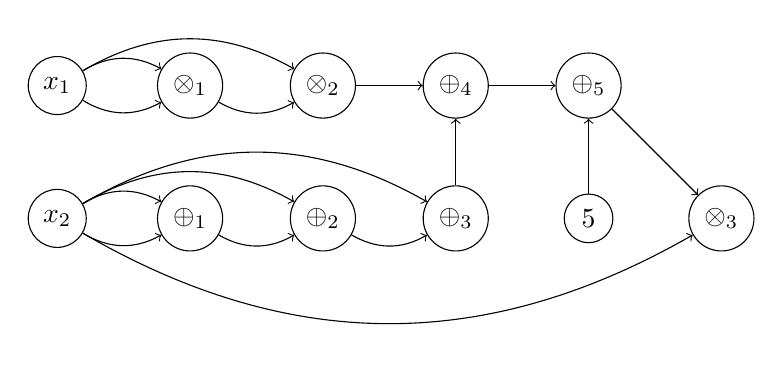
\begin{tikzpicture}[node distance={48pt}, node/.style = {draw, circle}]
		\node[node] (x1) {\(x_1\)};
		\node[node] (x2) [below of=x1] {\(x_2\)};
		\node[node] (m1) [right of=x1] {\(\otimes_1\)};
		\node[node] (m2) [right of=m1] {\(\otimes_2\)};
		\node[node] (a1) [right of=x2] {\(\oplus_1\)};
		\node[node] (a2) [right of=a1] {\(\oplus_2\)};
		\node[node] (a3) [right of=a2] {\(\oplus_3\)};
		\node[node] (a4) [right of=m2] {\(\oplus_4\)};
		\node[node] (a5) [right of=a4] {\(\oplus_5\)};
		\node[node] (5) [below of=a5] {\(5\)};
		\node[node] (m3) [right of=5] {\(\otimes_3\)};
		\draw[->] (x1) to [bend left] (m1);
		\draw[->] (x1) to [bend right] (m1);
		\draw[->] (x1) to [bend left] (m2);
		\draw[->] (m1) to [bend right] (m2);
		\draw[->] (x2) to [bend left] (a1);
		\draw[->] (x2) to [bend left] (a2);
		\draw[->] (x2) to [bend left] (a3);
		\draw[->] (x2) to [bend right] (a1);
		\draw[->] (a1) to [bend right] (a2);
		\draw[->] (a2) to [bend right] (a3);
		\draw[->] (m2) to (a4);
		\draw[->] (a3) to (a4);
		\draw[->] (a4) to (a5);
		\draw[->] (5) to (a5);
		\draw[->] (a5) to (m3);
		\draw[->] (x2) to [bend right] (m3);

	\end{tikzpicture}
	\caption{Arithmetic circuit of the formula shown in 
    \Cref{ex:arithmetic_formula}.}\label{fig:arithmetic_circuit}
\end{figure}

Since arithmetic circuits contain no cycles, they can only be used to represent a fixed number 
of operations (aka \emph{bounded computations}).
In general though, this is not really a big issue, as oftentimes we can easily synthesize circuits 
\emph{on-the-fly}.

Every arithmetic circuit can be then associated with a set of \emph{circuit assignments}.
\begin{definition}[Circuit assignment]
  A circuit assignment over an arithmetic circuit \(\mathcal{G} = \Tuple{V, E, L}\) is a triple 
  \(\mathcal{A}_{\mathcal{G}} = \Tuple{V, E, L'}\) such that, 
  \(\forall v \in V\colon \call{L'}{v} \in A\)
\end{definition}


\chapter{An Overview of Proof Systems}\label{chap:computation}
Proving theorems is an activity which has always been considered highly intellectual, and 
even today most theorems are proven ``by hand''. 
But what does it really mean to prove a theorem? Is finding a proof for a theorem really harder 
than checking whether said proof is valid? And is it possible to prove to someone that a theorem is 
true, without revealing why that is so?

In this chapter, after introducing the required concepts \emph{computation and complexity theory} 
in \Cref{sec:interactive_tm} and \Cref{sec:complexity}, we give an overview of 
\emph{interactive proof systems} in \Cref{sec:interactive_proof_systems}, and the history 
of their \emph{zero-knowledge} counterparts in \Cref{sec:zero_knowledge}.

\section{Interactive Turing machines}\label{sec:interactive_tm}
A \emph{computational model} (or model of computation) is any kind of system able to describe 
how to produce some \emph{output} given some \emph{input}~\cite{Savage1997}.
Different models do this in different ways, each one with its own strength and weaknesses in terms
of \emph{expressivness}, \emph{complexity} and \emph{succintness}.
Two historically important models of computations are Alonzo Church's 
\emph{\(\lambda \)-calculus}~\cite{Church1941} and Alan Turing's 
\emph{Turing machine} (TM)~\cite{Turing1950}. 
Among several equivalent models~\cite{Davis2004}, Turing machines became the standard model of 
computation.
\begin{definition}[Turing machine~\cite{Papadimitriou1994}]\label{def:turing_machine}
  A Turing machine is a quadruple \(\mathcal{M} = \Tuple{\Sigma, Q, q_0, \delta}\), where 
  the \emph{alphabet} \(\Sigma \) is a set of symbols such that \(\sqcup \in \Sigma \), the 
  \emph{state set} \(Q\) is a set of symbols such that \(\Set{\bot, \top} \subseteq Q\), 
  \(q_0 \in Q\) is the \emph{initial state}, and 
  \(\delta\colon {\Parens*{Q \setminus \Set{\bot, \top}} \times \Sigma} \to 
  {Q \times \Sigma \times \Set{\leftarrow, \rightarrow}}\) is the \emph{transition function}.
\end{definition}

By only requiring \(\delta \) to be a relation instead of a function, we obtain the so-called 
\emph{non-deterministic} Turing machine (NTM): given a state and an alphabet symbol, the machine 
can take different choiches at every step.
A TM \(\mathcal{M}\) manipulates a string \(\overbar{\sigma}\) over the alphabet 
\(\Sigma \setminus \Set{\sqcup}\) by placing it over an \emph{infinite, discrete working tape} 
\(\Tapework \), a total order isomorphic to \(\mathbb{Z}\).
The input string is positioned such that its first symbol is matched with the position \(0\) 
of the tape; all the positions before the first symbol and after the last symbol are filled 
with the \emph{blank} symbol \(\sqcup \).
The computation \(\call{\mathcal{M}}{\overbar{\sigma}}\) starts in the initial state \(q_0\) with 
the \emph{head} of the TM positioned over the position \(0\) of the tape, and proceeds according to 
the transition function: depending on the current state \(q\) and the symbol \(\sigma \) written in 
the current location of the head, it replaces \(\sigma \) with a new symbol \(\sigma'\), it moves 
the head to the left (\(\leftarrow \)) or to the right (\(\rightarrow \)) and it transitions into a 
new state \(q'\).
The computation \emph{terminates} whenever one of the two \emph{halting} states is reached: if
\(\call{\mathcal{M}}{\overbar{\sigma}} = \bot \), then the input string \(\overbar{\sigma}\) is 
\emph{rejected}, else if \(\call{\mathcal{M}}{\overbar{\sigma}} = \top \), then \(\overbar{\sigma}\) 
is \emph{accepted}.
It can also happen that the computation does not terminate: in such cases, we write 
\(\call{\mathcal{M}}{\overbar{\sigma}} = {\uparrow}\) and we say that the computation \emph{hangs}.

In many scenarios, it is useful to extend Turing machines to include additional features, for 
example to represent the ability to access some source of randomness, or to communicate with an 
external environment to read inputs and produce outputs in an interactive manner.
\begin{definition}[Input/Output Turing machine]
  An input/output Turing machine is a quadruple \(\mathcal{M} = \Tuple{\Sigma, Q, q_0, \delta}\)
  where \(\Sigma \), \(Q\) and \(q_0\) are defined as in \Cref{def:turing_machine}, and:
  \[
    \delta\colon {\Parens*{Q \setminus \Set{\bot, \top}} \times \Sigma^2} \to 
    {Q \times \Sigma^2 \times \Set{\leftarrow, \rightarrow}^2}
  \]  
\end{definition}

The additional parameters in the transition function of an input/output Turing machine (I/O TM) 
account for two new tapes, namely the \emph{read-only input tape} \(\Tapein \) and the 
\emph{write-only output tape} \(\Tapeout \): now, depending on the state \(q\), the input symbol 
\(\sigma_{i}\) and the working symbol \(\sigma_{w}\), the machine overwrites \(\sigma_{w}\) with a 
new symbol \(\sigma'_{w}\) and moves left/right on \(\Tapework \), it writes a new symbol 
\(\sigma_{o}\) on \(\Tapeout \), where it can move only to the right, and it moves to the 
left/right on \(\Tapein \).
Additionally, in an I/O TM, the input string is placed on \(\Tapein \) instead of \(\Tapework \), 
which is instead blank at the beginning of the computation.
\begin{definition}[Probabilistic Turing machine]
  A probabilistic Turing machine is a quadruple \(\mathcal{M} = \Tuple{\Sigma, Q, q_0, \delta}\)
  where \(\Sigma \), \(Q\) and \(q_0\) are defined as in \Cref{def:turing_machine}, and:
  \[
    \delta\colon {\Parens*{Q \setminus \Set{\bot, \top}} \times \Sigma \times \Set{0, 1}} \to 
    {Q \times \Sigma \times \Set{\leftarrow, \rightarrow}}
  \]    
\end{definition}

In a probabilistic Turing machine (PTM), we have an additional \emph{read-only random tape} 
\(\Taperand \) which is populated with an infinite, uniformly random sequence of \emph{coin tosses} 
(zeros and ones), that are used by the transition function to decide what to do.
As for the writing tape of an I/O TM, the head on \(\Taperand \) can only move to the right.
\begin{definition}[Interactive Turing machine]
  An interactive Turing machine is a quadruple \(\mathcal{M} = \Tuple{\Sigma, Q, q_0, \delta}\)
  where \(\Sigma \), \(Q\) and \(q_0\) are defined as in \Cref{def:turing_machine}, and:
  \[
    \delta\colon {\Parens*{Q \setminus \Set{\bot, \top}} \times \Sigma^2} \to
    {Q \times \Sigma^2 \times \Set{\leftarrow, \rightarrow}}
  \]
\end{definition}

An interactive Turing machine (ITM) is quite similar to an I/O TM, as it also has two additional 
tapes, called the \emph{send tape} \(\Tapesend \) and the \emph{receive tape} \(\Taperec \).
However, unlike for the input tape \(\Tapein \) of an I/O TM, the head on \(\Taperec \) cannot move 
backwards.
\begin{remark}  
  Our definition of ITM differs slightly from the standard one in the 
  literature~\cite{GoldreichMW1991,GoldwasserMR1989}, but we find it to be more modular.
  In any case, from now on, we will say \emph{interactive Turing machine} to actually mean an 
 \emph{interactive, probabilistic, input/output Turing machine}.
\end{remark}

\begin{definition}[Interactive protocol]
  An interactive protocol is a pair \(\mathcal{I} = \Tuple{\mathcal{M}, \mathcal{M'}}\)
  where \(\mathcal{M}\) and \(\mathcal{M'}\) are interactive Turing machines such that 
  \(\Tapein = \Tapein'\), \(\Tapesend = \Taperec' \), \(\Taperec = \Tapesend'\), and their 
  state sets \(Q, Q'\) contain the special \emph{idle state} \(q_{idle} \in Q, Q'\).
\end{definition}

The computation of an interactive protocol (IP) over some string \(\overbar{\sigma}\), 
\(\call{\mathcal{I}}{\overbar{\sigma}}\), proceeds in the following manner: 
initially, the tapes \(\Tapesend \), \(\Taperec \), \(\Tapework \), \(\Tapework' \), \(\Tapeout \) 
and \(\Tapeout' \) are all empty (i.e.\ filled with blank symbols), the tapes \(\Taperand \) and 
\(\Taperand' \) are filled with random bits, and the tape \(\Tapein \) contains \(\overbar{\sigma}\).
The ITM \(\mathcal{M}\) is said to be \emph{active} and works normally until it transitions in the 
special state \(q_{idle}\), becoming \emph{inactive}.
When this happens, control passes to \(\mathcal{M}'\), which becomes active and works normally 
until it reaches its own idle state; control goes back to \(\mathcal{M}\), and the process repeats.
When one of the two machines halts, control passes over the other one until it also halts.
The protocol \emph{succeeds} if both machines halt in the accepting state \(\top \), and it 
\emph{fails} if at least one of them halts in the rejecting state \(\bot \).
To denote the final states reached by one of the machines at the end of the computation, 
we write \(\call{\mathcal{I}_{\mathcal{M}}}{\overbar{\sigma}}\) and 
\(\call{\mathcal{I}_{\mathcal{M}'}}{\overbar{\sigma}}\) respectively.
\Cref{fig:interactive_protocol} depicts the fundamental structure of an interactive protocol.

\begin{figure}
  \centering
  \begin{tikzpicture}[node distance=64pt,on grid,auto]
    \node[state,shape=rectangle,minimum height=16pt, minimum width=48pt] (in)  {\(\Tapein = \Tapein'\)};
    \node[state,shape=rectangle,minimum size=24pt,left =of in]   (m0)         {\(\mathcal{M}\)};
    \node[state,shape=rectangle,minimum size=24pt,right =of in] (m1)  {\(\mathcal{M}'\)};
    \node[state,shape=rectangle,minimum height=16pt, minimum width=48pt,above left =of m0] (p0)  {\(\Taperand \)};
    \node[state,shape=rectangle,minimum height=16pt, minimum width=48pt,above right =of m1] (p1)  {\(\Taperand' \)};
    \node[state,shape=rectangle,minimum height=16pt, minimum width=48pt,below left =of m0] (w0)  {\(\Tapework \)};
    \node[state,shape=rectangle,minimum height=16pt, minimum width=48pt,below right =of m1] (w1)  {\(\Tapework' \)};
    \node[state,shape=rectangle,minimum height=16pt, minimum width=48pt,above =of in] (s0)  {\(\Tapesend = \Taperec' \)};
    \node[state,shape=rectangle,minimum height=16pt, minimum width=48pt,below =of in] (r0)  {\(\Taperec = \Tapesend' \)};
    \node[state,shape=rectangle,minimum height=16pt, minimum width=48pt,left =of m0] (o0)  {\(\Tapeout \)};
    \node[state,shape=rectangle,minimum height=16pt, minimum width=48pt,right =of m1] (o1)  {\(\Tapeout' \)};
    \path[->]
    (in) edge (m0)
    (in) edge (m1)
    (p0) edge (m0)
    (p1) edge (m1)
    (w0) edge (m0)
    (m0) edge (w0)
    (w1) edge (m1)
    (m1) edge (w1)
    (m0) edge (s0)
    (s0) edge (m1)
    (m1) edge (r0)
    (r0) edge (m0)
    (m0) edge (o0)
    (m1) edge (o1)
    ;
  \end{tikzpicture}
  \caption{Visualization of an interactive protocol.}\label{fig:interactive_protocol}
\end{figure}

\section{Problems and complexity}\label{sec:complexity}
Historically, the most important class of problems that have been analyzed are so-called
\emph{decision problems}, i.e.\ probles whose solution is a binary \emph{yes-or-no} 
answer~\cite{Sipser2013}.
This perfectly suits Turing machiens as we can interpret their acceptance or rejection of the input 
string respectively as a yes and a no answer.

\begin{definition}[Kleene's closure]
  The Kleene's closure of a set \(S\) is the set \(S^* = \bigcup_{n \in \mathbb{N}}{S^n}\).
\end{definition}

As Turing machine operate over strings in \(\Sigma^*\), also called \emph{words}, they partition 
\(\Sigma^* \) into three \emph{languages} (a language is any set of strings): the language of 
accepted words, the languages of rejected words and the language of hanging words.
\begin{definition}[Turing-recognizable language]
  A language \(L \subseteq \Sigma^*\) is recognized by some Turing machine \(\mathcal{M}\) if 
  \(\forall w \in L\colon \call{\mathcal{M}}{w} = \top \).
\end{definition}
\begin{definition}[Turing-decidable language]
  A language \(L \subseteq \Sigma^*\) is decided by some Turing machine \(\mathcal{M}\) if it is 
  recognized by \(\mathcal{M}\) and \(\forall w \notin L\colon \call{\mathcal{M}}{w} = \bot \).
\end{definition}

We denote the language recognized by a Turing machine \(\mathcal{M}\) with \(\call{L}{\mathcal{M}}\).
To solve an \emph{instance} \(\Pi \) of some decision problem \textsc{prob}, we first encode the 
instance into a string \(\Encode{\Pi} \in \Sigma^*\) such that 
\(\Encode{\Pi} \in \call{L}{\mathcal{M}}\) if and only if the answer to \(\Pi \) is `yes'.

The class of recognizable languages, called \textsc{RE}, strictly includes the class of decidable 
languages, called \textsc{DEC}~\cite{Turing1937}.
But even decidable languages are not all equal: their \emph{computational complexity}, that is,
the amount of some resource which is required by a Turing machine to decide membership words in 
function of their length, can vary wildly.
In general, we are only interested in the \emph{asymptotic behaviour} of the machine.
\begin{definition}[Big-O notation]
  Given two functions \(f, g\colon \mathbb{N} \to \mathbb{N}\), then \(f = \BigO{g}\) if 
  and only if \(\exists c,n\) such that \(\forall x \ge n\) \(\call{f}{x} \le c \cdot \call{g}{x}\).
\end{definition}

We write \(f = \BigOmega{g}\) when \(g = \BigO{f}\), and we write \(f = \BigTheta{g}\) when 
\(f = \BigO{g}\) and \(g = \BigO{f}\).
When there exists a TM \(\mathcal{M}\) for which some complexity metric \(\Complexity \) is 
upper-bounded at most by a polynomial function in the length \(n\) of the input word 
(i.e.\  \(\call{\Complexity}{\mathcal{M}} = \BigO{n^c}\) for some constant \(c \in \mathbb{N}\)), 
we say that deciding the language is \emph{feasible} w.r.t.\  \(\Complexity \). 
On the other hand, if \(\Complexity \) is upper-bounded at least by an 
exponential function (i.e.\  \(\call{\Complexity}{\mathcal{M}} = \BigO{c^{n}}\) for some constant 
\(c > 1\)), we say that the problem is \emph{infeasible} w.r.t.\  \(\Complexity \).
The standard complexity metrics are \emph{time} \(\Time \), that is the amount of transition steps 
a TM performs before halting, and \emph{space} \(\Space \), that is the amount of tape locations 
visited by a TM before halting\footnote{It is always the case that \(\Space \le \Time \).}.

Two of the most important 
\emph{complexity classes}\footnote{\url{https://complexityzoo.net/Complexity_Zoo}} 
are \textsc{PTIME} (\Ptime{} for short) and \textsc{NPTIME} (\NPtime{} for short), which are the 
classes of languages decidable respectively by a deterministic TM and a nondeterministic TM using 
at most polynomial time.
While we do not know if \(\Ptime \maybeequals \NPtime \), it is widely believed that 
\(\Ptime \subset \NPtime \): for a deterministic Turing machine, deciding \NPcomplete{} problems 
(i.e.\ the hardest problems in \NPtime{}) will generally take an exponential amount of 
time, and there is no known way in the physical world to build non-deterministic Turing machines.
Although quantum computers have been shown to be able to crack problems which are believed to 
be infeasible for standard computers, like integer factorization~\cite{Shor1994}, \NPcomplete{}
problems seem to be out of reach also for such powerful machines.

\section{Interactive proof systems}
Even though \NPcomplete{} problems are infeasible, they are \emph{efficient} to \emph{verify}: 
given an \emph{instance} \(\Pi \) of some \NPcomplete{} problem, and an additional \emph{witness}
string, we can build a deterministic TM that checks whether the witness \emph{proves} or 
not that the problem admits a positive answer.
\begin{example}
  Consider the problem \textsc{sat} of deciding whether a propositional logic formula \(\phi \) is 
  satisfiable, which is the most famous \NPcomplete{} problem~\cite{Cook1971}. 
  If we had a TM \(\mathcal{M}\) with access to an \emph{oracle} that, in \(\BigO{1}\) time, 
  provides a valid assignment for the variables in \(\phi \), it would be easy to 
  verify that \(\phi \) is indeed satisfiable.
  However, if the provided assignment was not valid, while \(\mathcal{M}\) would reject it, 
  there would be still no easy way to know whether \(\phi \) is actually satisfiable or not! 
\end{example}

Now, let's say we want to prove some theorem \(\Pi \): computationally, this is equivalent to 
deciding whether \(\Pi \) is word which belongs to the language of the valid propositions over some 
formal system (say, the ZFC set theory~\cite{FraenkelHL1973}).
A \emph{proof} of the theorem plays the same role of the \emph{witness} we discussed before: in 
general, verifying a proof for a theorem is (believed to be) much easier than finding the proof in 
the first place.
Hence, we can extend the logical/mathematical concept of theorem to the more computational concept 
of language: for example, by \NPtime{} theorem, we mean any language in \NPtime{}.

\clearpage
\begin{definition}[Interactive proof system~\cite{GoldwasserMR1989}]  
  An interactive proof system for a language \(L\) is an interactive protocol 
  \(\mathcal{I} = \Tuple{\mathcal{P}, \mathcal{V}}\), where \(\mathcal{P}\) is the \emph{prover}
  and \(\mathcal{V}\) is the \emph{verifier}, such that:
  \begin{align*}
    & \forall w \in L\colon \call{\mathcal{I}_{\mathcal{V}}}{w} = \top & 
      \textnormal{(\emph{correctness})} \\
    & \forall w \notin L\colon \call{\mathcal{I}_{\mathcal{V}}}{w} = \bot & 
      \textnormal{(\emph{completeness})} \\
    & \exists k \in \mathbb{N}\colon \call{\Time}{\mathcal{V}} = \BigO{\abs{x}^k} & 
    \textnormal{(\emph{boundness})}
  \end{align*}
\end{definition}

In an interactive proof system (IPS), the common input tape of \(\mathcal{P}\) and \(\mathcal{V}\)
contains some word \(w\) representing some statement: in typical scenario, the statement is 
provided by the prover himself, who wants to convince the verifier of the truthness of such 
statement.
During the protocol, \(\mathcal{P}\) and \(\mathcal{V}\) exchange messages through their 
communication tapes; at some point, \(\mathcal{P}\) sends to \(\mathcal{V}\) a candidate proof 
\(\pi \): the verifier checks the proof and, if the proof is valid, it is always convinced of its 
validity (correctness), hence it will accept. 
On the other hand, if the proof happens to be wrong (e.g.\ if \(\mathcal{P}\) is trying to deceive
\(\mathcal{V}\)), then the verifier will never be convinced by such a proof, and it will reject.
The polynomial bound on the execution time of \(\mathcal{V}\) is necessary to force cooperation, 
and avoid the case where \(\mathcal{V}\) simply ignores \(\mathcal{P}\) and computes the proof by 
itself.
\begin{definition}[Probabilistic interactive proof system~\cite{GoldwasserMR1989}]  
  A probabilistic interactive proof system for a language \(L\) is an interactive protocol 
  \(\mathcal{I} = \Tuple{\mathcal{P}, \mathcal{V}}\) such that, for any arbitrarily small 
  \(\epsilon \in \mathbb{R}_{+}\):
  \begin{align*}
    & \forall w \in L\colon \call{\Pr}{\call{\mathcal{I}_{\mathcal{V}}}{w} = \bot} < \epsilon  & 
      \textnormal{(\emph{probabilistic correctness})} \\
    & \forall w \notin L\colon \call{\Pr}{\call{\mathcal{I}_{\mathcal{V}}}{w} = \top} < \epsilon & 
      \textnormal{(\emph{probabilistic completeness})} \\
    & \exists k \in \mathbb{N}\colon \call{\Time}{\mathcal{V}} = \BigO{\abs{x}^k} & 
    \textnormal{(\emph{boundness})}
  \end{align*}
\end{definition}

\section{Zero-Knowledge Protocols}
Suppose that two parties are executing an IARK system for some hard problem: the instance is places 
on the shared input tape, and also suppose that the secret in possession of the prover is simply 
a witness for the instance. 
All the prover has to do is send the witness to the verifier, which will in turn check it and 
decide whether to accept or not.
In this process, the verifier gained more knowledge than just the solvability of the problem: it 
also learned a solution, and not just any solution, but exactly the one available to the prover,
which should have been a secret.
To address this issue, researchers started exploring the field of so-called zero-knowledge 
proofs~\cite{GoldwasserMR1989,GoldreichMW1991}.

Informally, two random variables \(U\) and \(V\) that map words of some language 
\(L \subseteq \Set{0, 1}^{*}\) to words of \(\Set{0, 1}^{*}\) are 
\emph{perfectly indistinguishable} when no unbounded Turing machine is able to tell them apart,
are \emph{statistically indistinguishable} when no \textsc{PSPACE} Turing machine is able to 
tell them apart, and are \emph{computationally indistinguishable} when no \textsc{PTIME} Turing 
machine \(\mathcal{M}\) is able to tell them apart.
By `telling apart', we mean that the distribution of the words that are accepted/rejected 
by Turing machines respecting the imposed bounds is independent from \(U\) and \(V\): intuitively,
this means that \(U\) and \(V\) are interchangable with each other and using one over the other 
does not give an `edge' to \(\mathcal{M}\)~\cite{GoldwasserM1984,GoldwasserMR1989,Yao1982}.
\begin{example}
  Consider the two random variables \(U, V: L \to \Set{0, 1}^{*}\) for some 
  \(L \subseteq \Set{0, 1}^{*}\), such that, for all words \(x \in L\) and all words 
  \(w \in \Set{0, 1}^{\abs{x}}\), it holds that:
  \begin{align*}
    & \call{\Pr}{\call{U}{x} = w} = 2^{-\abs{x}} &&
    \call{\Pr}{\call{V}{x} = w} = \begin{cases}
      0 & x = 0\dots0 \\
      2^{-\abs{x} + 1} & x = 1\dots1 \\
      2^{-\abs{x}} & \textrm{otherwise}
    \end{cases}
  \end{align*}
  \(U\) and \(V\) have \emph{almost} the same distribution, with the \(1\dots1\) string 
  happening twice as often in \(V\). 
  For increasingly longer strings, no Turing machine can tell the two distributions apart by 
  collecting a polynomial amount of samples, since 
  \(\sum_{w}{\abs{\call{\Pr}{\call{U}{x} = w} - \call{\Pr}{\call{V}{x} = w}}} = 2^{-\abs{x}+1}\),
  hence \(U\) and \(V\) are statistically indistinguishable.
\end{example}

\begin{definition}[Tape view]
  A \emph{tape view} is a random variable \(\View_{\mathcal{M}}\) that models the concatenation 
  of all the contents that are read/written by a halting Turing machine \(\mathcal{M}\) over its 
  tapes.
\end{definition}

For a deterministic, non-probabilistic Turing machine, the tape view variable is quite pointless, 
but it is a useful tool to model the behaviour of machines that exploit randomness, and expecially 
for interactive protocols.
For example, if we have a Turing machine with one tape \(\Tape \), then:
\[
  \call{\Pr}{\call{\View_{\mathcal{M}}}{x} = w} = 
  \call{\Pr}{\call{\View_{\mathcal{M}, \Tape}}{x} = w} = 
  \call{\Pr}{\call{\mathcal{M}}{x} = w}
\]


\begin{definition}[Approximability]
  A random variable \(U\) is (perfectly, statistically, computationally) \emph{approximable} by a 
  probabilistic Turing machine \(\mathcal{M}\) over some language \(L\) if \(U\) and 
  \(\View_{\mathcal{M}}\) are (perfectly, statistically, computationally) indistinguishable.
\end{definition}

Note that for a random variable \(U\) and a halting PTM \(\mathcal{M}\) to be perfectly 
indistinguishable over some language \(L\), it must be the case that 
\(\forall x \in L\colon \call{\mathcal{M}}{x} = \call{\View_{\mathcal{M}}}{x} = \call{\mathcal{U}}{x}\).

\begin{definition}[Zero-knowledge interactive protocol]
  A (perfectly, statistically, computationally) \emph{Zero-knowledge interactive protocol} (ZKIP) 
  over a language \(L \subseteq \Set{0, 1}^{*}\) is an interactive protocol 
  \(\mathcal{I} = \Tuple{\mathcal{M}, \mathcal{M}'}\) such that, for every \(\mathcal{M'}\),
  \(\View_{\mathcal{M'}}\) is (perfectly, statistically, computationally) approximable by a 
  Turing machine \(\mathcal{M}''\) over the language 
  \(L' = \Set{\Tuple{x, h} \mid x \in L \wedge w \in \Set{0, 1}^*}\), where the string
  \(h\) represents the initial content of \(\Tapework'\).
\end{definition}

Naturally, a ZKIP which is also a proof system is a zero-knowledge proof system (ZKPS); similarly, 
if it is an interactive argument of knowledge system then it is a zero-knowledge interactive 
argument of knowledge system (ZK-IARK).
From now on, by zero-knowledge we mean computational zero-knowledge, as assuming a polynomial-time 
bounded adversary is an acceptable restriction in the real world.
The initial string \(h\) of a ZKIP can be interpreted as the \emph{history} of previous 
interactions with the prover, or some eavesdropped information from the interactions that the 
prover had with other verifiers.

A proof system being zero-knowledge basically means that, even for curious or malicious verifiers,
and even with additional knowledge on the behaviour of the prover, what can be computed is nothing 
more than what could have been computed in polynomial time, hence within the imposed computational 
power limits, without communicating with the prover.
While it is obvious that every problem solvable in probabilistic polynomial time 
(\textsc{PP}) has a zero-knowledge proof system (the prover does nothing and the verifier computes 
the solution by himself), it was proven that also all problems in \textsc{NP} have a 
ZKPS~\cite{GoldreichMW1991}. 
By assuming the existance of secure probabilistic encryption, it was finally shown that also 
all Arthur-Merlin games, and hence all problems in \textsc{IP}, have a ZKPS~\cite{BenorGGHKMR1990}.

\subsection{Non interactive Zero-Knowledge}\label{subsec:nizk}
In many scenarios, especially ones involving multiple parties, interaction can be a problem as
the communication cost of bidirectional \(n\)-to-\(n\) grows quadratically.
Such cases are in fact of great interest for zero-knowledge systems: multiple parties can be 
both provers and/or verifiers, and their number might be huge.

For this reason, researches explored the possibility of having zero knowledge \emph{non-interactive} 
proof systems (ZK-NPS) or argument of knowledge systems (ZK-NARK).
Unfortunately, only the languages in \textsc{BPP}, that is languages decidable in 
probabilistic polynomial time with a bounded error allow for zero-knowledge non-interactive 
proofs~\cite{Oren1987,GoldreichK1996}. Such languages are of course trivial, as the verifier has 
enough power to do all the computation by itself without the need of the prover.

However, by introducing an initial \emph{preprocessing} phase, it is possible to regain the lost 
power~\cite{SantisMP1990}, and the most prominent technique to achieve non-interaction is the 
\emph{Common Reference String} (CRS) model~\cite{BlumFM1988} (sometimes also called 
\emph{common random string} model).
The main idea of the CRS model is that, before engaging in the protocol, the prover and 
the verifier have both obtained access to a shared string of random bits. 
In the simplest case, the string is generated by a \emph{trusted third party}, although in 
practice this is oftentimes not a viable solution as the whole point of zero-knowledge is having 
to deal with untrusted parties. 
To circumnent this problem, it is possible to generate the CRS by a \emph{majority vote}
between \(n\) authorities, which can be untrusted if picked singularly, but are assumed to be 
honest in their majority~\cite{GrothO2006}.
In fact, it was shown that it is possible, without losing zero-knowledge, to re-use multiple times 
a single CRS both by a single~\cite{BlumSMP1991} or multiple~\cite{FeigeLS1990} provers, although 
only for arguments of knowledge and not for proofs.

The first zero-knowledge systems, both interactive and non-interactive, were tailor-made for 
specific problems, such as the quadratic residuosity problem \textsc{qr}~\cite{GoldwasserMR1989}, 
the hamiltonian path problem \textsc{hampath}~\cite{LapidotS1991}, or the \(3\)-\textsc{sat} 
problem~\cite{BlumSMP1991}.
Although for any \textsc{NP-complete} problem \textsc{prob} there is a polynomial-time 
algorithm~\cite{Karp1972} that converts every instance of \textsc{prob} to an instance 
of, say, \(3\)-\textsc{sat}, such reductions are often not trivial to devise and very expensive 
to apply.
For this reason, researchers started devising constructions to prove arbitrary NP statements 
embedded in the form of boolean circuits~\cite{Damgard1993}, which can neatly represent the 
computation of a Turing machine over any \textsc{NP-complete} problem~\cite{Cook1971}, and 
therefore remove the need to go through polynomial-time reductions.

The first of such systems~\cite{Damgard1993} required a CRS of size cubic in the length of the 
statement to be proven, although XOR and NOT gates didn't need to consume any bits from the CRS\@.
In the following years, many improvements were proposed, reducing the complexity of the 
constructions from cubic to subquadratic~\cite{BoyarBP1995} and eventually 
linear~\cite{CramerD1997}.


\chapter{Cryptographical Background}\label{chap:crypto}
The main application of Zero Knowledge proof systems has been, arguably unsurprisingly, in the 
cryptography field.
The possibility of two or more parties to cooperate and exchange information one with another in a 
zero-knowledge manner is the fundamental idea behind many branches of cryptography such as 
\emph{Multi Party Computation} (MPC)~\cite{Yao1982-2} and \emph{Fully Homomorphic Encryption} 
(FHE)~\cite{ArmknechtEtAl2015}.

The main application of Zero knowledge protocols has been in \emph{blockchain} infrastructures, 
with the cryptocurrency \emph{ZCash} being the most prominent example~\cite{SassonCGGMTV2014}.
In a public blockchain, a user (the prover) wants to convince the other users (the verifiers) that 
he posseses some data: to this end, he exhibits a \emph{commitment}, typically a short message 
which can be easily computed when knowing the original data, but for which it is hard to find a 
\emph{collision}.
In this scenario, the prover would like to be able to convince the verifiers of the validity of 
its commitment, without having to hand them out the original data.

\chapter{Cryptographic Primitives from Generalized Triangular Dynamical Systems}\label{chap:arion}
One of the most important applications of zero-knowledge verifiable computation lies in digital 
currency transactions over the blockchain infrastructure.
An example of ZK-SNARK applied in the real world is the ZCash cryptocurrency~\cite{SassonCGGMTV2014}, 
which is inspired by the more famous Bitcoin~\cite{NarayananBFMG2016}, and was devised by the 
authors of \texttt{libsnark} (which frames the zero-knowledge backend of the currency).

As we discussed in \Cref{sec:tree_hash}, the fundamental component of a blockchain is the 
Merkle tree, which uses one-way compression functions in order to produce the binding 
commitment.
In a digital currency scenario, the leaves of the Merkle tree consist of the details of some 
transaction, typical information include the ID of the sender, the ID of the recipient, and the 
amount of currency to be transferred. 
Without a zero-knowledge framework in place, when one wants to verify whether a user did abide to 
their commitment, the only possible solution is to ask the user to disclose his transaction, 
together with the authentication path, and check that the tree commitment is respected. 
When using currencies like Bitcoin or Ethereum\footnote{\url{https://ethereum.org/}}, anyone 
can see the details of every single transaction being performed on the relative 
blockchain, meaning that there is no privacy whatsoever\footnote{For example, on 
\url{https://etherscan.io/} you can see the transactions on the Ethereum blockchain. %It is 
%curious how privacy has often been foisted as a feature of mainstream cryptocurrencies while, 
%on the contrary, any bank offers much more privacy!
}.
However, if we translate the Merkle tree computation in an equivalent circuit, it is possible to 
apply a zero-knowledge scheme that allows a verifier to be sure (with overwhelming probability) 
of the validity of a transaction without actually having to see it!
Since a Merkle tree applies over and over the underlying compression function, the problem of 
creating a circuit for the former immediately reduces to the problem of creating a circuit for the 
latter.

In \Cref{sec:sota} we will review the evolution of the state of the art concerning zero-knowledge 
friendly compression functions.
Then, in \Cref{sec:gtds}, we present a new algebraic framework to represent cryptographic 
primitives, the \emph{Generalized Triangular Dynamic System}, and apply it to construct the 
\Arion{} block cipher and the \Arionhash{} hash function.
Finally, in \Cref{sec:performance}, we compare our new construction to the state of the art using 
the \texttt{libsnark} library, showing extremely competitive results.
\input{parts/hash/arion/sota.tex}
\input{parts/hash/arion/gtds.tex}
\input{parts/hash/arion/performance.tex}

\section{Tree-like modes of hashing}\label{sec:tree_hash}
Consider an \(n\)-bit CHF \(H\), and suppose that a prover claims to know some message \(m\): 
the digest \(d = \call{H}{m}\) can be considered as a \emph{short binding commitment} for \(m\): 
By asking the prover to share the digest, whose size \(\abs{d} = n\) is typically considered to be 
\(\BigO{1}\) (or \(\BigO{\call{\log}{\abs{m}}}\) in some cases), a verifier is convinced that the 
prover does know \(m\) with probability \(\approx 1 - {1}/{2^n}\).
A modern standard CHF like SHA-256~\cite{Dang2015} produces digests of length at least \(256\) bits,
making the \(1 - {1}/{2^n}\) bound really hard to bruteforce through.
Note that the verifier needs not to know \(m\) in advance: the commitment \(d\) is (temporarily) 
appended to a public \emph{blockchain} and, at any point in the future, when the verifier becomes 
aware of some \(m'\) provided by the prover, if \(\call{H}{m'} = d\), the commitment can be 
approved or rejected.

Now, suppose that the prover wants to commit to a list of \(k\) messages: the simplest solution 
would be to publish the hash of every message, which would require to append \(\BigO{k}\) 
elements on the blockchain.
Another way would be for the prover to share \(\call{H}{\Tuple{m_1, \dots, m_k}}\): the 
communication cost would only be \(\BigO{1}\) but, in general, not all the messages belong to the 
same prover, so this method would not work, and we need a better solution.

\subsection{Merkle tree}
\begin{definition}[Binary Merkle tree~\cite{Merkle1988}]
	A \emph{binary Merkle tree (MT)} of height \(h \in \mathbb{N}\) over a \(2n\)-to-\(n\) compression 
	function \(C\), is the complete binary tree of height \(h\) such that, given a sequence of input 
	messages \(\Tuple{m_1, \dots, m_{2^{h-1}}}\) over \(\Set{0, 1}^{2n}\), produces an
	output digest \(d \in \Set{0, 1}^{n}\) in the following way:
	\begin{enumerate}
		\item The leaf nodes \(\nu_1, \dots, \nu_{2^{h-1}}\) contain 
					\(\call{C}{m_1}, \dots, \call{C}{m_{2^{h-1}}}\).
		\item Every other node \(\nu \) contains \(\call{C}{\nu_l, \nu_r}\), where \(\nu_l\) is
		      the left child of \(\nu \) and \(\nu_r\) is the right child of \(\nu \).
		\item The output digest \(d\) is the content of the root node. 
	\end{enumerate}
\end{definition}

The set of the sibling nodes visited in the path from a leaf of the tree to the root, including the 
leaf itself, is the \emph{authentication path} of the leaf.
By using Merkle trees, the prover only needs to send to the verifier, as a commitment for
some message \(m_i\) among \(n = 2^h\) messages, the contents of the co-path from the leaf 
containing \(m_i\) to the root, in addition plus the hash of \(m_i\): this requires
just \(\BigO{\call{\log}{n}}\) cost to validate the commitment.
Merkle trees bottom-up construction is very easy to parallelize, and they can be used in the 
multiple-provers scenario: each prover only needs to commit to the path from its own leaf to the 
root of the tree.
It is immediate to generalize the notion of binary Merkle tree to arbitrary arity.
\begin{proposition}[Security of Merkle tree mode of hash~\cite{Merkle1988}]
	Given a one-way \(tn\)-to-\(n\) compression function \(C\), the \(t\)-ary Merkle tree over 
	\(C\) is a cryptographic hash function.
\end{proposition}

\begin{example}\label{ex:merkle_tree}
	Consider the sequence of pre-hashed messages \(S = \Tuple{3, 4, 7, 7}\) and the 
	compression function 
	\(\call{C}{x, y}: \Tuple{x, y} \mapsto \Parens*{xy \bmod 13} + 1\) (for ease of exposition, 
	we work over integers instead of bit strings, but the two can be readily converted into one 
	another).
	\Cref{fig:merkle_tree} shows the contents of the associated Merkle Tree.
	Note that the real message is not stored in the Merkle Tree, but only the `first level' of hashes.
	The authentication path of the leaf labelled with \(3\) consists of the tuple \(\Tuple{3, 4, 11}\):
	by computing \(\call{H}{3, 4} = 13\) and then \(\call{H}{13, 11} = 1\) we can verify that the 
	commitment is respected.
\end{example}
\begin{figure}
	\centering
	\begin{tikzpicture}[node distance={32pt}, node/.style = {draw, circle},on grid=true]
		\node[node] (x1) {\(3\)};
		\node[node,draw=none] (n1) [right of=x1] {};
		\node[node] (x2) [right of=n1] {\(4\)};
		\node[node,shape=rectangle] (c1) [above of=n1] {\(C\)};
		\node[node,draw=none] (n2) [right of=x2] {};
		\node[node] (x3) [right of=n2] {\(7\)};
		\node[node,draw=none] (n3) [right of=x3] {};
		\node[node] (x4) [right of=n3] {\(7\)};
		\node[node,shape=rectangle] (c2) [above of=n3] {\(C\)};
		\node[node] (x5) [above of=c1] {\(13\)};
		\node[node,draw=none] (n3) [above of=n2] {};
		\node[node,draw=none] (n4) [above of=n3] {};
		\node[node] (x6) [above of=c2] {\(11\)};
		\node[node,shape=rectangle] (c3) [above of=n4] {\(C\)};
		\node[node] (x7) [above of=c3] {\(1\)};
		\draw[->] (x1) to (c1);
		\draw[->] (x2) to (c1);
		\draw[->] (x3) to (c2);
		\draw[->] (x4) to (c2);
		\draw[->] (c1) to (x5);
		\draw[->] (c2) to (x6);
		\draw[->] (x5) to (c3);
		\draw[->] (x6) to (c3);
		\draw[->] (c3) to (x7);
	\end{tikzpicture}
	\caption{Merkle tree of \Cref{ex:merkle_tree}.}\label{fig:merkle_tree}
\end{figure}

\subsection{Augmented Binary Tree}
The Merkle tree is the de-facto standard for blockchain applications, and basically for any 
scenario for which a `linear' hash function cannot be used.
In~\cite{Stam2008}, it was given a lower bound on the amount of queries necessary to obtain a 
collision for a \(\Parens*{m+s}\)-to-\(s\)-bit CHF \(H\) (the \(m\) is variable) built from a 
\(\Parens*{n+c}\)-to-\(n\)-bit OWCF \(C\): if \(H\) makes \(r\) queries to \(C\), it is possible 
to find a collision by making \(2^{\frac{nr + cr - m}{r + 1}}\) queries to \(H\).
By combining this result with the \(2^{s/2}\) upper bound of the birthday paradox, one can 
immediately obtain a tight bound \(m = \frac{2nr + 2cr -sr - s}{2}\) for the variable length \(m\) 
of the message.

\begin{definition}[Compactness~\cite{AndreevaBR2021}]
	The \emph{compactness} of an \(\Parens*{m+s}\)-to-\(s\)-bit hash function making \(r\) queries to 
	an underlying \(\Parens*{n+c}\)-to-\(n\)-bit one-way compression function is the value
	\(\alpha = \frac{2m}{2nr + 2cr -sr - s}\).
\end{definition}

\begin{example}\label{ex:mtree_compactness}
	Consider a \(2n\)-to-\(n\) bit OWCF and a Merkle Tree of height \(h\): the computation 
	of the tree is a \(\Parens*{2^{h-1}n}\)-to-\(n\)-bit hash function, and makes exactly 
	\(r = 2^{h-1} - 1\) queries to \(C\).
	We have \(s = c = n\) and \(m = 2^{h-1}n - n = nr\), therefore the compactness of the Merkle 
	Tree construction is:
	\[
		\alpha = \frac{2m}{2nr + 2cr -sr - s} = 
		\frac{2nr}{2nr + 2nr - nr - n} =
		\frac{2r}{3r - 1}
	\]
	Which tends to \(2/3\) when \(r\) tends to infinity.
\end{example}

\begin{definition}[Augmented Binary tRee~\cite{AndreevaBR2021}]
	An \emph{Augmented Binary tRee (ABR)} of height \(h \in \mathbb{N}\) over a 
	\(2n\)-to\(n\) compression function \(C\) is a complete binary tree of height \(h\) 
	augmented with \emph{middle} nodes such that, given a sequence of input messages
	\(S = \Tuple{m_1, \dots, m_{2^{h-1} + 2^{h-2}-1} \mid \forall i\colon m_i \in \Set{0, 1}^{*}}\), 
	it produces an output digest \(d \in \Set{0, 1}^n\) in the following way:
	\begin{enumerate}
		\item The leaf nodes \(\nu_{1}, \dots, \nu_{2^{h-1}}\) contain \(\call{C}{m_1}, \dots,
		      \call{C}{m_{2^{h-1}}}\).
		\item There are no middle nodes in the leaf layer.
		\item The middle nodes \(\nu_{2^{h-1}+1}, \dots, \nu_{\abs{S}}\) contain
		      \(\call{C}{m_{2^{h-1}+1}}, \dots, \call{C}{m_{\abs{S}}}\).
		\item Every other node \(\nu \) contains \(\call{C}{\nu_l \oplus \nu_m, \nu_r \oplus
		      \nu_m} \oplus \nu_r \), where \(\nu_l\) is the left child of \(\nu \), \(\nu_r\)
		      is the right child of \(\nu \), and \(\nu_m\) is the middle child of \(\nu \), or \(0\)
		      if \(\nu \) doesen't have a middle child.
	\end{enumerate}
\end{definition}

The authentication path of the ABR is similar to the one of the Merkle tree, but also includes 
the middle nodes encountered during the traversal.

\begin{proposition}[Security of ABR mode of hash~\cite{AndreevaBR2021}]
	Given a one-way \(2n\)-to-\(n\) compression function \(C\), the ABR over \(C\) is a cryptographic 
	hash function.
\end{proposition}

An ABR of height \(h\) can process 50\% more messages than a Merkle Tree of the same height, 
while performing the same number of queries to the underlying compression function, with the 
additional cost introduced by the intermediate \(\oplus \) operations being negligible in most 
scenarios.

\begin{example}
	Consider a \(2n\)-to-\(n\) bit OWCF and an ABR of height \(h\): the computation 
	of the tree is a \(\Parens*{2^{h-1} + 2^{h-2}-1}n\)-to-\(n\)-bit hash function, 
	and makes exactly \(r = 2^{h-1} - 1\) queries to \(C\).
	Like in \Cref{ex:mtree_compactness}, we have \(s = c = n\), but this time 
	\(m = \Parens*{2^{h-1} + 2^{h-2}-1}n - n = nr + {nr}/2 - n\), so the compactness of the ABR 
	construction is:
	\[
		\alpha = \frac{2m}{2nr + 2cr - sr - s} = 
		\frac{2nr + nr - 2n}{2nr + 2nr - nr - n} =
		\frac{3r - 2}{3r - 1}
	\]
	Which approaches \(1\) as \(r\) approaches infinity, meaning that the ABR construction achieves
	optimal compactness.
\end{example}

It is worth of notice that, while the ABR hash mode achieves collision resistance, it does not 
achieve \emph{indifferentiability} (a weaker notion of indistinguishability between Turing 
machines~\cite{MaurerRH2003}), hence a modified construction, called ABR+, was also proposed, 
although it does not achieve perfect compactness.
\begin{figure}
	\centering
	\begin{tikzpicture}[node distance={32pt}, node/.style = {draw, circle},on grid=true]
		\node[node] (x1) {\(3\)};
		\node[node,draw=none] (n1) [right of=x1] {};
		\node[node] (x2) [right of=n1] {\(4\)};
		\node[node,shape=rectangle] (c1) [above of=n1] {\(C\)};
		\node[node,draw=none] (n2) [right of=x2] {};
		\node[node] (x3) [right of=n2] {\(7\)};
		\node[node,draw=none] (n3) [right of=x3] {};
		\node[node] (x4) [right of=n3] {\(7\)};
		\node[node,shape=rectangle] (c2) [above of=n3] {\(C\)};
		\node[node,draw=none] (n4) [above of=n2] {};
		\node[node] (x8) [above of=n4] {\(10\)};
		\node[node] (x5) [above of=c1] {\(13\)};
		\node[node] (x6) [above of=c2] {\(11\)};
		\node[node,draw=none] (n5) [above of=x8] {};
		\node[node,shape=rectangle] (c3) [above of=n5] {\(C\)};
		\node[node,shape=rectangle] (a1) [below left of=c3] {\(\oplus \)};
		\node[node,shape=rectangle] (a2) [below right of=c3] {\(\oplus \)};
		\node[node,shape=rectangle] (a3) [above of=c3] {\(\oplus \)};
		\node[node] (x7) [above of=a3] {\(10\)};
		\draw[->] (x1) to (c1);
		\draw[->] (x2) to (c1);
		\draw[->] (x3) to (c2);
		\draw[->] (x4) to (c2);
		\draw[->] (c1) to (x5);
		\draw[->] (c2) to (x6);
		\draw[->] (x5) to (a1);
		\draw[->] (x6) to (a2);
		\draw[->] (x8) to (a1);
		\draw[->] (x8) to (a2);
		\draw[->] (a1) to (c3);
		\draw[->] (a2) to (c3);
		\draw[->] (c3) to (a3);
		\draw[->] (x5) [bend left] to (a3);
		\draw[->] (a3) to (x7);
	\end{tikzpicture}
	\caption{ABR of \Cref{ex:abr}.}\label{fig:abr}
\end{figure}
\begin{example}\label{ex:abr}
	Consider the same compression function \(C\) of \Cref{ex:merkle_tree}, and consider the 
	sequence of pre-hashed messages \(S' = \Tuple{3, 4, 7, 7, 10}\), in this case we interpret 
	\(x \oplus y \equiv \Parens*{x + y \bmod 13} + 1\).
	\Cref{fig:abr} shows the resulting ABR\@.
	The authentication path of the node labelled with \(3\) consists of the tuple 
	\(\Tuple{3, 4, 10, 11}\): by computing \(\call{H}{3, 4} = 13\) and then 
	\(\call{H}{13 \oplus 10, 11 \oplus 10} \oplus 13 = 10\) we can verify that the commitment is 
	respected.
\end{example}

\section{ZK-SNARK systems}
As we saw in \Cref{subsec:nizk}, researchers were able to construct ZK-NARK systems whose 
verification complexity was linear in the size of the problem instance, which is provided as a 
boolean circuit.
Furthermore, in the CRS model, by using a block cipher, it is also possible to have 
\emph{publicly verifiable} constructions~\cite{LapidotS1991}, meaning that \emph{any} verifier, 
not just the one that engages the protocol, is able to check the proof, which is encrypted with a 
\emph{proving key}, by using a public \emph{verification key}.

\begin{proposition}[Fiat-Shamir heuristic~\cite{FiatS1987}]
  Suppose a probabilistic I/O TM \(\mathcal{P}\) with access to a CHF \(H\) wants to prove its 
  knowledge of the discrete logarithm \(x = \call{\log}{y}\) for some value 
  \(y \in \mathbb{Z}_p\), where \(p\) is a large prime number.
  Then \(\mathcal{P}\) can sample a random value \(v\) from \(\Taperand \), compute the digest 
  \(d = \call{H}{p, y, p^v}\), the result \(r = {v - dx} \bmod \Parens*{p - 1}\), and finally 
  output the quadruple \(\Tuple{p, y, p^v, r}\).
  Any \textnormal{\textsc{PTIME}} TM \(\mathcal{V}\) with access to \(\Tuple{p, y, p^v, r}\) 
  and \(H\) can recompute \(d\) and check whether \(p^v = p^{r}y^{d}\)
  (If \(\mathcal{P}\) is not cheating, then \(p^{r}y^{d} = p^{v - dx}\Parens*{p^{x}}^d = 
  p^{v - dx}p^{dx} = p^{v - dx + dx} = p^v\)).
  Assuming that the discrete logarithm is hard and that true CHF exist, if equality holds 
  \(\mathcal{V}\) is convinced that \(\mathcal{P}\) knows \(x\) but is not able to retrieve it 
  except with negligible probability.
\end{proposition}

\begin{definition}[Succint proof]
  A \emph{succint proof} for a statement \(\sigma \) over a language \(L \subseteq \Set{0, 1}^*\) 
  is a proof \(\pi \) such that \(\abs{\pi} = \BigO{\call{\log}{\abs{\sigma}}}\).
\end{definition}

Similarly, one can define the notion of succint argument of knowledge, and in particular, a 
succint ZK-NARK system is called a ZK-SNARK system.
\begin{definition}[Probabilistically checkable proof system~\cite{BabaiFLS1991,FeigeGLSS1991}]
  A \emph{probabilistically checkable proof system} (PCP system) is an interactive proof system 
  \(\Tuple{\mathcal{P, V}}\) such that for any proof \(\pi \) provided by \(\mathcal{P}\):
  \(\exists k\colon \call{\Time}{\mathcal{V}} = \BigO{\call{\log^k}{\abs{\pi}}}\).
\end{definition}

In a PCP system, the prover \(\mathcal{P}\) constructs a proof \(\pi \) of size polynomial in the 
length of the original statement \(\sigma \); since the verifier \(\mathcal{V}\) is 
polylogarithmically bound to the size of the proof, it can only query a small portion of it, 
however, it is enough to get statistical completeness and soundness.

In~\cite{Kilian1992}, the author uses Merkle trees to have the prover commit to a proof \(\pi \), 
(the bits of \(\pi \) are the leaves and the root, whcih has constant size, is sent to the verifier). 
The verifier then queries a certain number of authentication paths, which have length
\(\BigO{\call{\log}{\abs{\pi}}}\), and decides whether to accept or reject.
In this sense, the protocol is therefore succint.
In~\cite{Micali2000}, the construction was extended and, by applying the Fiat-Shamir heuristic, it 
is possible to make the protocol non-interactive.

One of the first \emph{succint} ZK-NARK (ZK-SNARK) systems that didn't make explicit use of 
PCPs was devised in~\cite{Groth2010}, but had one important drawback: while the size of the proof 
is constant, the size of the CRS, and the computation that the prover has to perform is 
\emph{quadratic} in the size of the input circuit
(this bound wass slightly improved in~\cite{Lipmaa2011}).

However, by first transforming the circuit into \emph{quadratic span programs} (QSPs), 
the boolean equivalent of QAPs (\Cref{subsec:qap}), it was possible to reduce both the size of the 
CRS and the prover's computational complexity to linear, while still having succint proofs.
Since all these constructions make use of encryption based on the hardness of finding the discrete
logarithm of a number over a big finite field, dealing with boolean circuits and QSPs is not 
very efficient; although both polynomially sized boolean and arithmetic circuits are equivalent to 
\textsc{PTIME} Turing machines~\cite{PippengerF1979}, working over arithmetic programs, and hence 
using R1CSs~\cite{CramerD1998} and QAPs over QSPs, can greatly reduce the constant factors involved 
in such constructions, although this depends on the kind of input problem (numeric problems 
can exploit arithmetic circuits much better than, say, propositional problems).

\subsection{Pinocchio}
An important application of ZK-SNARK systems is in \emph{verifiable computation}.
Consider a client (say, a mobile phone) that wants to delegate to a server (say, a cloud provider) 
some computation, for which several inputs are required: some are provided by the client, 
and some by the server:
\begin{itemize}
  \item The client does not trust the server, so we would need a proof system, but since the server 
        is not computationally unbounded, an \emph{argument of knowledge} system will suffice.
  \item The server might have to interact with many clients or, similarly, many different clients
        might require the same computation, the system must be \emph{non-interactive}.
  \item Verifying the computation must be cheaper than performing it, otherwise the client wouldn't 
        have to ask the server in the first place, the system must provide \emph{succint} proofs.
  \item The server has too interests in to the client that the computation was correct, say to 
        avoid legal liability, but it is not willing to share its own inputs, so our system must
        be \emph{zero-knowledge}.
\end{itemize}
Clearly, among the various constructions we saw up to now, ZK-SNARK systems are the only one that 
can reasonably fulfill all these requirements.
However, all the constructions we saw, due to the high overheads involved 
(generating the CRS, building the QSP/QAP, generating the proof, etc.), were not efficient enough 
to make the whole process faster than just letting the client perform the computations by itself.

The first construction that was efficient enough to be practically usable was 
\emph{Pinocchio}~\cite{ParnoGHR2013}.


\subsection{Groth16}
\subsection{PLONK}


